% !TEX TS-program = xelatex
% !TEX encoding = UTF-8
\documentclass[a4paper, 12pt]{amsart}
\renewcommand\baselinestretch{1.5}
\usepackage{xeCJK, amsthm, tikz, algorithm, algorithmicx, algpseudocode,  amsaddr, hyperref}
%\usepackage[notref, notcite]{showkeys}
\setCJKmainfont[ItalicFont={KaiTi}, BoldFont={SimHei}]{SimSun}
\setCJKsansfont{SimHei}
\setCJKmonofont{FangSong}
\xeCJKsetup{AutoFakeSlant={true}, AutoFakeBold={true}}
\newcommand{\md}{\mathrm{d}}
\newcommand{\lr}[1]{\left(#1\right)}
\newcommand{\abs}[1]{\left\lvert#1\right\rvert}
\newcommand{\nm}[2]{\left\|\,#1\,\right\|_{#2}}
\newcommand{\set}[2]{\left\{\,#1\,\mid\,#2\,\right\}}
\newcommand{\sgn}{\mathrm{sgn}}
\newcommand{\minmod}{\mathrm{minmod}}
\numberwithin{equation}{section}
%\theoremstyle{definition}
\newtheorem{theorem}{定理}[section]
\newtheorem{prop}[theorem]{命题}
\renewcommand\proofname{\bf 证明. }
%\renewcommand\emailaddrname{电子邮箱: }
\renewcommand\datename{时间: }
\renewcommand\tablename{表}
\renewcommand\figurename{图}
\floatname{algorithm}{算法}
\renewcommand{\algorithmicrequire}{\bf 输入: }
\renewcommand{\algorithmicensure}{\bf 输出: }

\begin{document}
\title[TVD Methods for Burgers Equations]{\Large Burgers 方程的TVD格式求解}
\author[Y.L. Liao]{廖钰蕾}
\address{数学与系统科学研究院计算数学与科学工程计算研究所\\
电子邮箱 {\tt: \url{liaoyulei19@mails.ucas.ac.cn}}
}
%\email{liaoyulei19@mails.ucas.ac.cn}
\date{2019年12月11日}
\maketitle

\section{\large\bf 问题描述}
对无粘的Burgers 方程的
\[u_t+(u^2/2)_x=0,\]
考虑两种初值:
\begin{enumerate}
\item 光滑初值$u_1(x)=\sin(\pi x),x\in[0,2]$, 周期边界条件.
\item 间断初值:
\[u_2(x)=\begin{cases}
1,\quad&x\le0,\\
-0.5,\quad&x>0.
\end{cases}\]
\end{enumerate}
分别使用
\begin{enumerate}
\item Lax-Friedrichs 格式,
\item Godunov 格式,
\item 无$f'(u)\ge0$条件假设的MUSCL 格式,
\item Kurganov-Tadmor格式(推广的MUSCL格式)
\end{enumerate}
求解.
\begin{enumerate}
\item 计算各个格式分别对光滑解和间断解的$L^1$收敛阶数.
\item 对于解出现间断的情况, 选一个合适的网格大小和迭代终止时刻, 将精确解和数值解画在同一个图中进行直观比较.
\end{enumerate}

\section{\large\bf 关键算法和格式}
\subsection{第一种初值精确解求解方法}\hspace*{\fill}\par
利用特征线可以计算Burgers方程的精确解. 第一种初值问题的解仅在$x=1$处出现激波, 无稀疏波, 特征线如图~\ref{fig:chr}所示.
\begin{figure}[htbp]\centering\begin{tikzpicture}
\draw[->](-2.5,0)--(2.5,0);
\node[below]at(2.5,0){$x$};
\draw[->](-2,-0.5)--(-2,1.5);
\node[left]at(-2,1.5){$t$};
\node[below left]at(-2,0){0};
\node[left]at(-2,1){0.5};
\draw[->](-2,0)--(-2,1);
\node[below]at(0,0){1};
\draw[->](-1.5,0)--(-0.8,1);
\draw[->](-1,0)--(0,1);
\node[below]at(-1,0){0.5};
\draw[->](-0.5,0)--(0,0.7);
\draw[->](0.5,0)--(0,0.7);
\draw[->](1,0)--(0,1);
\node[below]at(1,0){1.5};
\draw[->](1.5,0)--(0.8,1);
\draw[->](2,0)--(2,1);
\node[below]at(2,0){2};
\end{tikzpicture}\caption{第一种初值的特征线}\label{fig:chr}\end{figure}

若点$(x,t)$处精确解为$u$, 则过该点的特征线$x'=x+u(t'-t)$交$t_0=0$于点$x_0=x-ut$处, 且在$(x_0,0)$处的精确解$u_1(x-ut)=\sin(\pi(x-ut))$. 故点$(x,t)$处精确解$u$满足方程
\[f(u):=u-\sin(\pi(x-ut))=0.\]

我们采用Newton 迭代法计算点$(x,t)$处精确解$u$. 由图~\ref{fig:chr}特征线可以看出, 对于给定$t\ge0.5$时, \[\set{x_0=x-ut}{0\le x\le2}\subset\left[0,\dfrac12\right]\cup\left[\dfrac32,2\right].\]
因此算法中迭代初值选用
\begin{equation}\label{eq:init}u(x,t)=\begin{cases}
\sin(\pi x),\quad&t<0.5,\\
\sgn(1-x)\sin(\pi x/2),\quad&t\ge0.5.
\end{cases}\end{equation}
其中$\sgn(\cdot)$为符号函数.

\subsection{第二种初值精确解}\hspace*{\fill}\par
利用特征线可以计算Burgers方程的精确解. 第二种初值问题的解在$x=t/4$处出现激波, 方程的解为
\[u(x,t)\begin{cases}
1,\quad&x\le t/4,\\
-0.5,\quad&x>t/4.
\end{cases}\]


\subsection{数值解计算格式}\hspace*{\fill}\par
定义
\begin{align*}
\minmod(a,b)&:=\begin{cases}
a,\quad&\abs{a}\le\abs{b},ab>0,\\
b,\quad&\abs{b}<\abs{a},ab>0,\\
0,\quad&ab\le0,
\end{cases}\\
\minmod(a,b,c)&:=\minmod(a,\minmod(b,c)).
\end{align*}

对于Burgers 方程$f(u)=u^2/2$, 数值格式如下:
\begin{itemize}
\item Lax-Friedrichs:
\begin{align*}
\Hat{f}_{j+1/2}&=\dfrac12\lr{\dfrac12u_j^2+\dfrac12u_{j+1}^2-\lr{u_{j+1}-u_j}},\\
u_j^{n+1}&=u_j^n-\dfrac{\Delta t}{\Delta x}\lr{\Hat{f}_{j+1/2}-\Hat{f}_{j-1/2}}.
\end{align*}
由于$\max\abs{f'}=1$.
\item Godunov:
\begin{align*}
\Hat{f}_{j+1/2}&=\begin{cases}
\min(u_j^2,u_{j+1}^2)/2,\quad&u_j<u_{j+1}\text{ 且 }u_{j}u_{j+1}>0,\\
\max(u_j^2,u_{j+1}^2)/2,\quad&u_j\ge u_{j+1},\\
0,\quad&\text{否则}.
\end{cases}\\
u_j^{n+1}&=u_j^n-\dfrac{\Delta t}{\Delta x}\lr{\Hat{f}_{j+1/2}-\Hat{f}_{j-1/2}}.
\end{align*}
\item MUSCL:
定义迭代算子
\[G_j(u):=u_j-\dfrac{\Delta t}{\Delta x}\lr{\Hat{f}(u_{j+1/2}^{-},u_{j+1/2}^{+})-\Hat{f}(u_{j-1/2}^{-},u_{j-1/2}^{+})},\]
其中$\Hat{f}(\uparrow,\downarrow)$为单调通量, 
\begin{align*}
\Tilde{u}_j&:=\dfrac12\minmod(u_{j+1}-u_j,u_j-u_{j-1}),\\
u_{j+1/2}^{-}&:=u_j+\Tilde{u}_j,\quad u_{j+1/2}^{+}:=u_{j+1}-\Tilde{u}_{j+1},
\end{align*}
采用2阶Runge-Kutta格式
\begin{align*}
u^{(1)}&=G(u^n),\\
u^{n+1}&=\dfrac12\lr{u^n+G(u^{(1)})}.
\end{align*}
\item Kurganov-Tadmor:
定义迭代算子
\[G_j(u):=u_j-\dfrac{\Delta t}{\Delta x}\lr{\Hat{f}(u_{j+1/2}^{-,mod},u_{j+1/2}^{+,mod})-\Hat{f}(u_{j-1/2}^{-,mod},u_{j-1/2}^{+,mod})},\]
其中$\Hat{f}(\uparrow,\downarrow)$为单调通量, 
\begin{align*}
u_{j+1/2}^{-}&:=-\dfrac16u_{j-1}+\dfrac56u_j+\dfrac13u_{j+1},\\
u_{j+1/2}^{+}&:=\dfrac13u_j+\dfrac56u_{j+1}-\dfrac16u_{j+2},\\
\Tilde{u}_j^{mod}&:=\minmod(u_{j+1/2}^{-}-u_j,u_{j+1}-u_j,u_j-u_{j-1}),\\
\Tilde{\Tilde{u}}_j^{mod}&:=\minmod(u_j-u_{j-1/2}^{+},u_{j+1}-u_j,u_j-u_{j-1}),\\
u_{j+1/2}^{-,mod}&:=u_j+\Tilde{u}_j^{mod},\quad u_{j+1/2}^{+,mod}:=u_{j+1}-\Tilde{\Tilde{u}}_{j+1}^{mod},
\end{align*}
采用3阶Runge-Kutta格式
\begin{align*}
u^{(1)}&=G(u^n),\\
u^{(2)}&=\dfrac34u^n+\dfrac14G(u^{(1)}),\\
u^{n+1}&=\dfrac13u^n+\dfrac23G(u^{(2)}).
\end{align*}
\end{itemize}

待求问题为初值问题, 不含边界条件. 因此在第$n+1$次迭代中, 将第$n$次数值解$u_j^n,j=1,\cdots,N$延拓到$u_j^n,j=-1,0,1,\cdots,N,N+1,N+2$. 具体地, 对于第一种初值, 由初值的周期性可知每层数值解也是周期的, 即$u_{-1}=u_{N-2},u_0=u_{N-1},u_{N+1}=u_2,u_{N+2}=u_3$. 对于第二种初值, 当激波没有超出边界时, $u_{-1}=u_0=1,u_{N+1}=u_{N+2}=-0.5$.

\section{\large\bf 数值实验}
实验使用GNU Octave v5.1.0~\footnote{\url{https://www.gnu.org/software/octave/doc/v5.1.0/}}实现, 运行系统为Windows10-x64. 第一种初值选取区域$x\in[0,2]$, 第二种初值选取区域$x\in[-1,1]$.

由于$\max\abs{f'}=\max\lvert\partial_1\Hat{f}\rvert=\max\lvert\partial_2\Hat{f}\rvert=1$, 实验中我们取$\Delta t/\Delta x=1/4$. 计算精确解$u$时, Newton 迭代法的终止条件为$\nm{f(u)}{\infty}\le\text{1e-10}$. MUSCL 与Kurganov-Tadmor 格式的单调通量选用Lax-Friedrichs通量
\[\Hat{f}(u^{-},u^{+})=\dfrac12\lr{\dfrac12(u^{-})^2+\dfrac12(u^{+})^2-\lr{u^{+}-u^{-}}}.\]

\subsection{第一个数值实验}\hspace*{\fill}\par
我们计算$t=0.15$时上述五种TVD格式的$L^1$误差和收敛阶, 第一种初值实验结果见表~\ref{tab:task1}, 其中表头为网格细度$\Delta x$的值. 由表中结果可以看出, 对于光滑初值问题, Lax-Friedrichs, Godunov 的误差较大, 收敛阶为1. MUSCL, Kurganov-Tadmor 的误差较小, 其中MUSCL 收敛阶为2, Kurganov-Tadmor 的实验收敛阶为2.2. Kurganov-Tadmor 格式收敛阶没有到3, 我们认为原因是其格式用小区域的平均值代替格点值, 这里会有2阶精度损失.
\begin{table}[htbp]\centering\caption{第一种初值$L^1$误差和收敛阶, 表头为$\Delta x$的值}\label{tab:task1}
\begin{tabular}{ccccccc}
\hline\hline
1/20 & 1/40 & 1/80 & 1/160 & 1/320 & 1/640\\
\hline\hline
\multicolumn{6}{l}{Lax-Friedrichs}\\
4.924e-2 & 2.514e-2 & 1.269e-2 & 6.371e-3 & 3.192e-3 & 1.597e-3\\
rate & 0.97 & 0.99 & 0.99 & 1.00 & 1.00\\ 
\hline
\multicolumn{6}{l}{Godunov}\\
3.201e-2 & 1.797e-2 & 9.572e-3 & 4.947e-3 & 2.516e-3 & 1.269e-3\\
rate & 0.83 & 0.91 & 0.95 & 0.98 & 0.99\\
\hline
\multicolumn{6}{l}{MUSCL}\\
7.770e-3 & 2.113e-3 & 5.997e-4 & 1.623e-4 & 4.308e-5 & 1.131e-5\\
rate & 1.88 & 1.82 & 1.89 & 1.91 & 1.93\\
\hline
\multicolumn{6}{l}{Kurganov-Tadmor}\\
3.308e-3 & 7.779e-4 & 1.723e-4 & 3.655e-5 & 7.738e-6 & 1.708e-6\\
rate & 2.09 & 2.17 & 2.24 & 2.24 & 2.18\\
\hline\hline
\end{tabular}\end{table}

第二种初值实验结果见表~\ref{tab:task2}, 其中表头为网格细度$\Delta x$的值. 由表中结果可以看出, 对于间断初值问题, Lax-Friedrichs, Godunov, MUSCL, Kurganov-Tadmor 四种格式收敛阶均为1, 其中Godunov 格式误差最小, MUSCL, Kurganov-Tadmor 选用Lax-Friedrichs 通量, 误差相比Lax-Friedrichs 小.
\begin{table}[htbp]\centering\caption{第二种初值$L^1$误差和收敛阶, 表头为$\Delta x$的值}\label{tab:task2}
\begin{tabular}{ccccccc}
\hline\hline
1/20 & 1/40 & 1/80 & 1/160 & 1/320 & 1/640\\
\hline\hline
\multicolumn{6}{l}{Lax-Friedrichs}\\
7.302e-2 & 3.509e-2 & 1.673e-2 & 8.405e-3 & 4.203e-3 & 2.101e-3\\
rate & 1.06 & 1.07 & 0.99 & 1.00 & 1.00\\
\hline
\multicolumn{6}{l}{Godunov}\\
5.625e-2 & 1.954e-2 & 3.644e-3 & 1.822e-3 & 9.111e-4 & 4.556e-4\\
rate & 1.53 & 2.42 & 1.00 & 1.00 & 1.00\\
\hline
\multicolumn{6}{l}{MUSCL}\\
5.949e-2 & 1.347e-2 & 8.986e-3 & 4.493e-3 & 2.247e-3 & 1.123e-3\\
rate & 1.34 & 1.39 & 1.00 & 1.00 & 1.00\\
\hline
\multicolumn{6}{l}{Kurganov-Tadmor}\\
5.755e-2 & 2.088e-2 & 6.331e-3 & 3.165e-3 & 1.583e-3 & 7.913e-4\\
rate & 1.46 & 1.72 & 1.00 & 1.00 & 1.00\\
\hline\hline
\end{tabular}\end{table}

\subsection{第二个数值实验}\hspace*{\fill}\par
我们绘制了$t=0.5$时精确解和Lax-Friedrichs, Godunov, MUSCL, Kurganov-Tadmor 格式数值解对比图, 网格细度$\Delta t=1/256,\Delta x=1/64$. 第一种初值对比图见图~\ref{fig:task1}, 第二种初值对比图见图~\ref{fig:task2}. 可以看出无论是对光滑初值还是间断初值, 四种格式保持总变差不增. Lax-Wendroff格式相比其它格式误差略大.
\begin{figure}[htbp]\centering
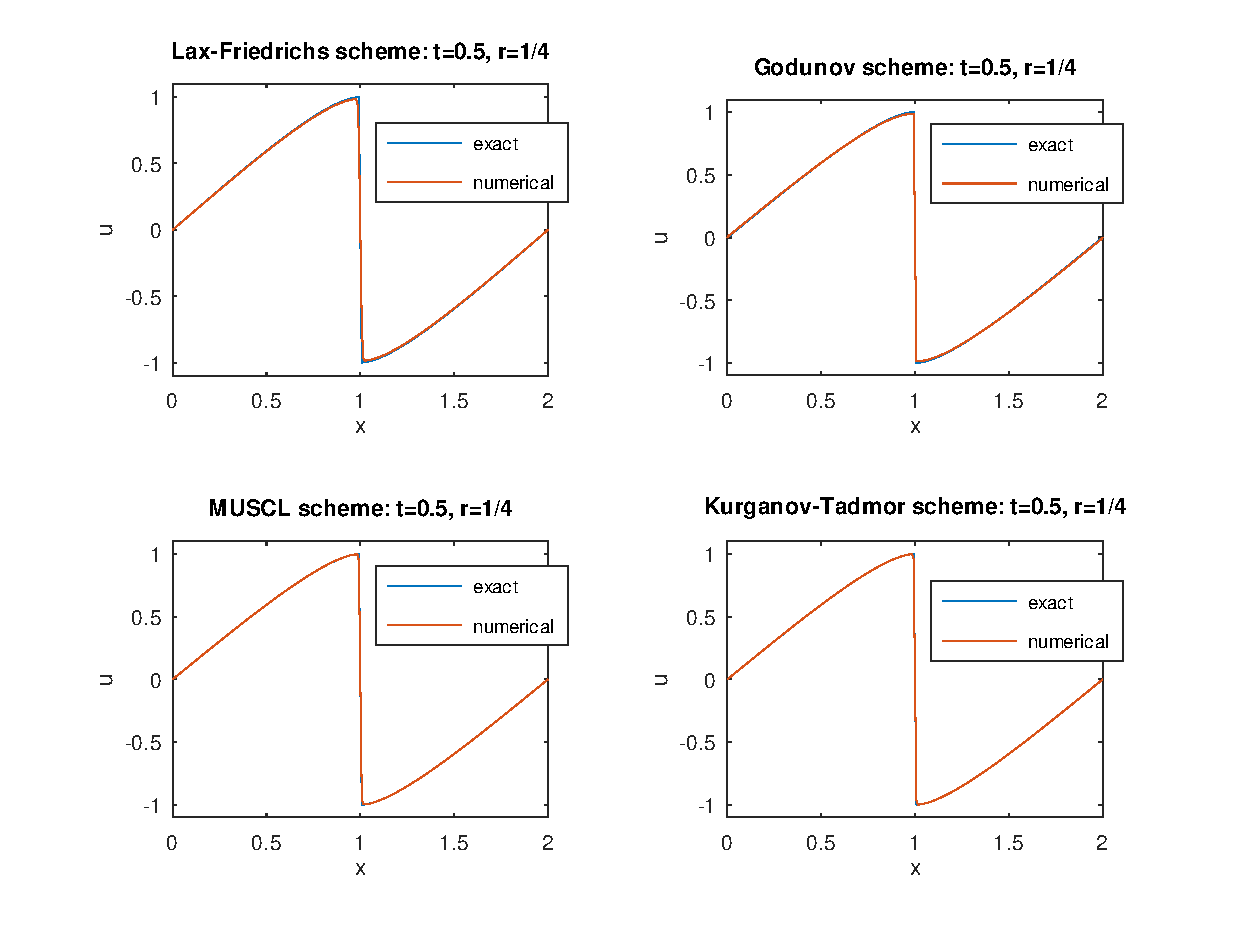
\includegraphics[width=\textwidth]{eq1.eps}
\caption{第一种初值的对比图}\label{fig:task1}
\end{figure}

\begin{figure}[htbp]\centering
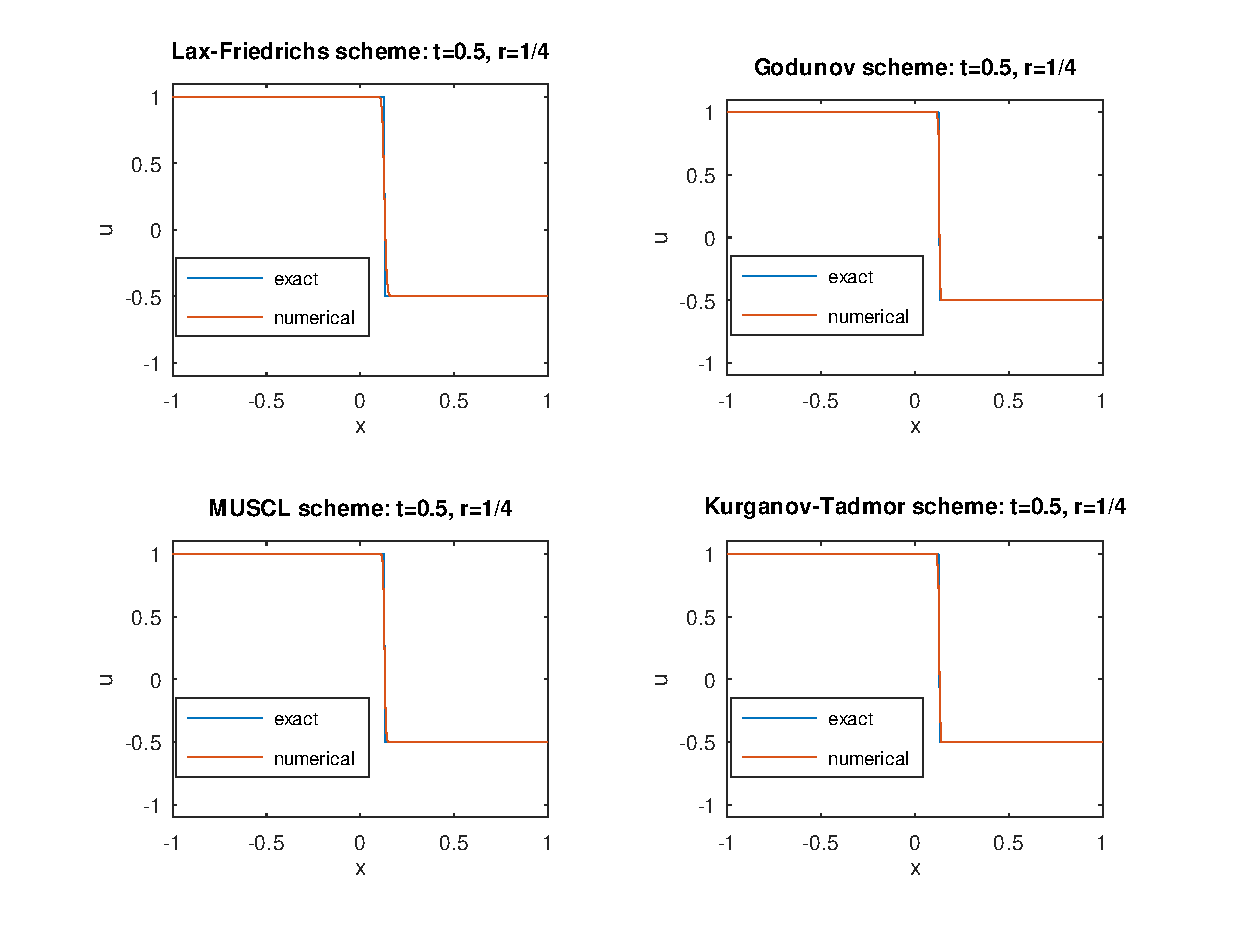
\includegraphics[width=\textwidth]{eq2.eps}
\caption{第二种初值的对比图}\label{fig:task2}
\end{figure}

\end{document}